\section{Findings}

\begin{figure*}
  \centering
  \includesvg[width=1.5\columnwidth]{images/ht_system.svg}
  \caption{The designed workflow for a \PC{} order. The client requests a worker through the smartphone app (1). \PC{}'s algorithm chooses a suitable worker (2) and rings them to see if they will take the order (3). If so, the client is called by customer support, to ensure the order is genuine (4). If it is, the worker receives a confirmation call from the system (5) and is asked to give an ETA and leave towards the client's house. During the journey, the worker is called up three times to get an updated ETA (6). Upon arrival, the worker calls the system to log the work as having started (7) and completes the job (8). After finishing, the worker calls into the system to log the work as finished (9). At any time, the worker can call the system to get information about a current job or their wages, get help from the \PC{} office or emergency services, or to contact the client (X). }~\label{fig:WorkFlow}
\end{figure*}

These findings are presented in relation to the specific points of the final \PC{} system design (illustrated in Figure \ref{fig:WorkFlow}) from the perspective of the domestic workers: ways in which they directly or indirectly engage with the system during a single `job cycle', from worker selection to the final sign-off after the job is complete. We outline the purpose and quality of the interactions between the domestic workers and the IVR system, drawing on recordings and notes from design discussions held between between the research team, \PC{}, and \NGO{} around the creation of the IVR interaction process. Through these observations, we reveal how the process of designing IVR system acted as a design probe: surfacing the diversity of values and motivations the three key stakeholders had in engaging with this process, as well as how these differences were negotiated and evident in the final design. 

\subsection{Being Selected for a Potential Job}

\begin{figure}[h]
  \centering
  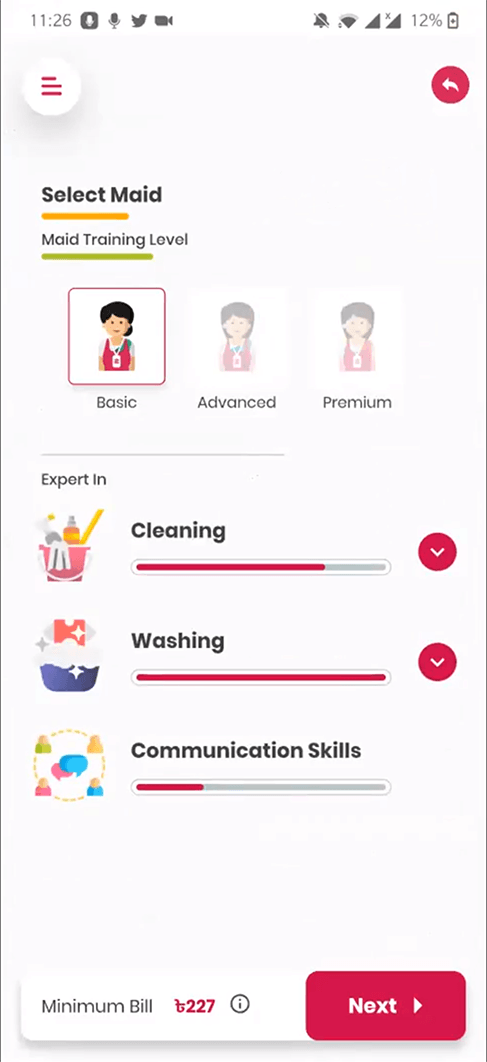
\includegraphics[width=0.65\linewidth]{images/orderingaworker.png}
  \caption{The interface the customer sees when ordering a worker through the \PC{} smartphone application.}\label{fig:Ordering}
  \Description{A screen of the \PC{} smartphone app, titled `Select Maid'. The user chooses a `maid training level', with the options `basic', `advanced' or `premium'. Several progress bars show the maid's purported skills: high in cleaning and washing, with lower communications skills. At the bottom of the screen is the minimum bill for this maid training level: 227 taka (around \$2.66 USD).}
\end{figure}

The job cycle begins with a client applying for a worker to come to their home through the \PC{} smartphone app. When ordering, users are asked how long they would like a maid for, and to choose how the level of training they require: with the options of `Basic', `Advanced' and `Premium' maids (Figure \ref{fig:Ordering}). Maids with a higher `training level' offer additional services such as cooking and additional communication skills (such as app use) at a higher rate of pay. The order confirmation screen clearly presents two conditions the user is required to agree to: i) that they must pay at least the paid amount for up to the requested length of time, and that additional time will cost extra; i)) that \PC{} `\textit{reserves the right to take legislative action on behalf of the victim(s) in case of verbal, physical or sexual abuse taking place to any party}.' 

When asked how the algorithm selected a specific worker for a job, \PC{} revealed that they were automatically sorted and prioritised based on the following factors:

\textbf{Proximity of worker to client:} the algorithm prioritises workers within a 1km radius of the client’s home, and then gradually extends out to 2-3km depending on availability.

\textbf{Worker's System Rating}:  workers are given a rating which reflects the frequency in which they accept or reject offers of work. All new workers start with a rating of 100 as a way to support new workers gaining a foothold in the \PC{} system. This rating declines every time a worker rejects the offer of a job:

\begin{displayquote}
\textbf{\PCTwo{}}: “If she performs well, it will be around that 100, 98 or 97. . . if she performs bad it will be dropping. This way, new domestic workers will always receive preference to be offered work."  
\end{displayquote}

\textbf{Worker's Client Rating}: clients rate workers using a five-star rating system. Clients are encouraged to rate workers highly if they would like to receive them again:

\begin{displayquote}
\textbf{\PCTwo{}}: "We are encouraging our clients to give 5 stars to his or her preferable domestic worker, and when a worker gets a five star from the client, she will be in first place [of the recommendation algorithm]"
\end{displayquote}

\textbf{Work History}: workers who have previously worked for a client will get priority with them:

\begin{displayquote}
\textbf{\PCTwo{}}:"If she has worked in this user’s house, it will give her an advantage because she knows the address."
\end{displayquote}

\textbf{Worker's Rating of the Client}: after completing a job, workers are able to leave ratings of the client. \NGOOne{} suggested that taking these ratings into account would help avoid malicious use of positive ratings from clients:

\begin{displayquote}
\textbf{\NGOOne{}}:"One rating will be from the employer’s side: if she gets five [stars] she’ll be called again. We are also taking ratings from the employee level---how she feels working there. Are you going to consider this? Because it might be that she might not be comfortable with working there: it might be that I’m a bad person, and give her five stars to get her again, but she’s not comfortable with me."

\textbf{\PCTwo{}}:"Yes. We should make it the first point---if the domestic worker does not want to go there, we should not consider her...”
\end{displayquote}

However, the algorithm in use during the `Human IVR' prototype did not take workers' reports about clients into account: 

\begin{displayquote}
\textbf{\PCTwo{}}: "It is not in action that the domestic worker will not get the same [client] if she doesn't want to, through a phone call, so we need to work on that."
\end{displayquote}


\subsection{Accepting the Job}

Once the algorithm has nominated a worker, they then receive an automated phone call about the job through the IVR system, saying:

\begin{displayquote}
\textit{You have a work request of [2] hours from [area name] and it will pay you [142] taka. The user's name is [Ishtiaque]. You [haven't] worked there previously. Press 1 to accept the order. Press 2 to reject the order. Press 3 to hear the order again.}
\end{displayquote}

If the worker rejects the order or if they hang up, the system will call the next worker prioritised by the algorithm. If they accept, they are played an audio recording detailing the exact location of the client's home, and asked to either reject the job or re-confirm it by giving an estimated time of arrival (ETA), with the options of 30 minutes, 60 minutes, or longer than 60 minutes.

Our design discussions with \PC{} revealed that the worker was given little access to information regarding both the client and the job when choosing whether or not to accept. For example, the IVR menu design did not give the worker information regarding the nature of the work (i.e. what they would be doing), the client's rating by other workers, or who will be present in the household during the work. In contrast, clients were given access to the worker's past ratings, a profile photo, phone number, and their `Training Level'. Some of these omissions could be explained by the limitations of IVR, the need for timeliness, and that logistical information about the job took priority. However, another stated concern was that the inclusion of additional information such as client ratings could `confuse' the workers:

\begin{displayquote}
\textbf{\PCTwo{}}: "The domestic worker might not understand the rating system to be able to assess the client. So I think we need to do the screening from the back end."
\end{displayquote}


\subsection{Confirming the Job}

After the worker accepts the job request they are asked to wait while a \PC{} customer support agent manually calls the client directly to confirm that the job is legitimate, and that the client isn't simply testing to see how the system works (this happens for every order, even with repeat customers). The worker then receives a second automated call saying that the job is legitimate:

\begin{displayquote}
\textit{Your order has been confirmed. Please set out for [Ishtiaque]’s house at [area]. Please only enter the user’s house if you see a woman in the house, wear a mask, and immediately report any safeguard issue by calling us. Call us back at [123456] whenever you need any support. To hear the user's detailed address, press 1. To talk to the user, press 2. To talk to the office, press 0. Otherwise, please hang up the call now and set off for the user’s house.}
\end{displayquote}

The contents of this message were informed by conditions set out by \NGO{}:

\begin{displayquote}
\textbf{\NGOOne{}}: "When the domestic worker gets the confirmation, she will be informed [to only work] if  there is a woman in the workplace, if she feels safe, and to always wear a mask. So three instructions will be there, so that we can take three actions to make her safer."
\end{displayquote}

When queried about why the domestic workers were called and engaged to a job prior to confirming with the client that the job is legitimate, \PC{} expressed that this process meant they could avoid cancelling on a client in an instance where they couldn't find a suitable worker:

\begin{displayquote}
\textbf{\PCTwo{}}: "We do not want to call the user without first confirming that we have a domestic worker in place to serve him. It will make him dissatisfied."
\end{displayquote}

\subsection{Travelling to the Job}

\subsection{Starting the Job}

\subsection{Completing the Job}

% --------------------------------------------------------------
% After a job request was received from a client, \PC{} needed to assign a domestic worker to fulfill it. In the designed IVR system, the process of deciding the most suitable worker was handled by an algorithm (Figure \ref{fig:WorkFlow}.2), and the chosen worker would receive an automated call offering them the job (Figure \ref{fig:WorkFlow}.3). After agreeing to take the job, the worker is asked to choose their estimated time of arrival (ETA) from multiple options, and told to wait for a confirmation phone call before leaving towards the client's house. Prior to this automated design, this was handled by the local guides, who would be given details of the job and asked to call and assign a suitable worker to it. However, the local guides' choices were not always in-line with PC's priorities:

% \begin{displayquote}
% \textbf{\PCTwo{}}: "When it was local guides, our service often saw failure when trying to get a domestic worker. It was not always within one or two kilometres: sometimes they always wanted workers to get to work, whether it is 1, 2 or even 3 kilometres. Or sometimes they used the logic that `\textit{I have to distribute the work equally---I have sent a domestic worker to a job in the morning, now, even though this new job is near that worker’s house, I will send another worker to distribute it equally.}’ But now, in our system you cannot do that."
% \end{displayquote}

% The \PC{} and \NGO{} stakeholders were also aware that this system was open to potential manipulation and exploitation by the local guides:

% \begin{displayquote}
% \textbf{\PCOne{}}: "When we had local guides in place, they assigned domestic workers manually, so there was always an option to manipulate: ‘\textit{Oh, I like this domestic worker, I want to give her the job.}’ [...] We provide the local guide with a list of ten domestic workers ordered based on the requirements, like from one to ten---the local guide can still assign the tenth domestic worker because it’s a manual process."
% \end{displayquote}

% Instead of relying on human decision making, the new system uses an algorithm which prioritised the workers based on their location, user rating, and system rating:

% \begin{displayquote}
% \textbf{\PCTwo{}}: "Firstly our app detects the domestic workers within a 1km radius of the customer’s home, and [then it takes into account] the rating by our users. [...] The next rating is the `system rating'. This is updated based on the responses from the domestic worker to offers of work: if she had been rejecting orders each and every time it will develop a bad rating for her. For new domestic workers---you raised this concern---they start with an initial rating of 100. If she performs well, it will be around that 100, 98 or 97… if she performs bad it will be dropping. This way, new domestic workers will always receive preference to be offered work."
% \end{displayquote}

% After a suggestion from \NGOOne{}, this was adapted to also take into account historical ratings of the client from workers: 

% \begin{displayquote}
% \textbf{\NGOOne{}}: "As [\PCTwo{}] mentioned, one rating will be from the employer’s side---if she gets five [stars] she’ll be called again. We are also taking ratings from the employee level: how she feels working there. Are you going to consider this? Because it might be that she might not be comfortable with working there---it might be that I’m a bad person, and give her five stars to get her again, but she’s not comfortable with me. So we need to..."

% \textbf{\PCTwo{}}: "Both sides of the coin. Yes. We should make it the first point: if the domestic worker does not want to go there, we should not consider her..."
% \end{displayquote}

% During the `human IVR' deployment, \PCTwo{} described the prototype's decision-making process as being `half human brain, half computer':

% \begin{displayquote}
% \textbf{\PCTwo{}}: "It was like a full human brain before---our [local guides] were using their brain to find a domestic worker, with slightly different logic. But now it is one human brain and one computer: the computer is receiving the order, is finding the domestic worker. The other human brain is just interacting after that---‘\textit{Ok, you are the chosen one}’---they’re getting a list of five or ten. They do not even know these domestic workers. I think it will just be the one computer when it is IVR, without the human brain. We are almost half way, or more than half way."
% \end{displayquote}

% However, the domestic workers reacted negatively to this new process, finding it limiting and uncomfortable to talk to a scripted stranger:

% \begin{displayquote}
% \textbf{\PCTwo{}}: "We have had some feedback. It was easier for them to interact with the `complete human brain’: they could interact in an unlimited way, but now it’s a limited logic, and they want to see the face of the customer support---they have seen the face of their local guide. So they used to feel at ease, but now they feel like they get a call from a random place, and they forget the order. Sometimes they even complain: ‘\textit{we can’t understand their language.}' It's not a problem of accent or language, it’s about thinking ‘\textit{I do not know him, so I do not get his message.}’"
% \end{displayquote}

% When the system calls the prioritised worker, it gives a basic overview of the job: the client's name, the area they live in, how long the job will take, and how much they will get paid. The research team suggested that the worker could also benefit from being informed of the client's rating by other domestic workers. \PC{} were initially hesitant, noting that the rating might confuse the workers, and opining that decisions about which clients should be served should be made by \PC{} in the back-end: 

% \begin{displayquote}
% \textbf{\PCTwo{}}: "Right, but I’m worried that the domestic worker might not understand the rating system to be able to assess the client. So I think we need to do the screening from the back end."
% \end{displayquote}

% Despite appearing to agree and them earlier noting that workers' wants should be considered, the feature didn't make it into the final design:

% \begin{displayquote}
% \textbf{R2}: "It doesn't have to be a number: it could be a word, like ‘\textit{this client has been rated excellent}’."

% \textbf{\PCTwo{}}: "Right. We could use a word, we could do that."
% \end{displayquote}


% \subsubsection{Confirming the Job}

% Once a worker has been found, one of PC's customer support agents then calls the client to confirm that the job is legitimate (Figure \ref{fig:WorkFlow}.4): \PCTwo{} noted that clients frequently create jobs within the smartphone app to test that the system works, and so these test jobs need to be identified before telling the assigned worker to leave for their house. They specified that this should even happen for repeat clients, not just ones new to the application. When we asked why this confirmation is made after first finding a worker, they noted that they didn't want to confirm with a legitimate customer only to then cancel the job if they couldn't find a suitable worker: 

% \begin{displayquote}
% \textbf{\PCTwo{}}: "We try to find a domestic worker for the required job first, and then we go to the user to confirm the order, because [...] we do not want to call the user without first confirming that we have a domestic worker in place to serve him. It will make him dissatisfied---we have called the user but then we won’t be able to provide a domestic worker. So, we want to make sure that we have a domestic worker in place so that if he or she wants to take the order, we can provide it."
% \end{displayquote}

% After confirming the job is legitimate, the worker will then receive a second automated `confirmation call' from the system (Figure \ref{fig:WorkFlow}.5). As a condition of their partnership, \NGO{} required that this confirmation call include a message outlining precautions which would assist in the worker's safety:

% \begin{displayquote}
% \textbf{\NGOOne{}}: "Know that [\PC{}] is practicing a very good thing with a few conditions: when the domestic worker gets the confirmation, she will be informed [to only work] if  there is a woman in the workplace, if she feels safe, and to always wear a mask. So three instructions will be there, so that we can take three actions to make her safer."
% \end{displayquote}

% For the `Human IVR' prototype, these warnings had been formalised into `checkpoints'---standards which the worker had been instructed to be sure had been met, otherwise they were instructed to call \PC{} to cancel the order and return home:

% \begin{displayquote}
% \textbf{\PCTwo{}}: "We have several ‘checkpoints’ when serving the order: whether it is a family house, whether a female member is present in the house while the worker will be working."
% \end{displayquote}

% \subsubsection{Tracking the Worker}

% While travelling to the client's house, the worker receives up to three automated `tracking calls' (Figure \ref{fig:WorkFlow}.6): the first is made 15 minutes after they received the confirmation call, and asks if the worker has left yet; another call is made after two thirds of the given ETA has expired, and asks for an updated ETA; and the final call is made 10 minutes after the ETA if the worker has not yet logged starting work. As the workers are likely to be departing from their own house, we queried if it's possible that they are likely to be in the middle of other tasks when orders come through, such as housework, cooking or childcare:

% \begin{displayquote}
% \textbf{\PCTwo{}}: "In our training, we’ll be telling them to ‘\textit{please be ready when you get an order call, and set out as soon as you get the confirmation call}’. So it’s our expectation that she’ll be ready and waiting for the confirmation call to get out. [...] We are training them to be done with all of their work from their end in the morning, and wait for the job all day long, we will be giving you one after one."
% \end{displayquote}

% We raised a concern that these calls are likely to feel intrusive, and asked for clarification on the intention behind them. \PCTwo{} claimed they were necessary in order to `push' the workers to get to the client on time: 

% \begin{displayquote}
% \textbf{\PCTwo{}}: If they have received an order we have to keep pushing them if she is already on the way, because we have to maintain a certain time---on the user’s side we have already committed them at the start of the order that it will take 30 minutes, 60 minutes, based on the estimation of the domestic worker. So we don’t need to make this [time] any longer than this, so we keep pushing them if they are already on the way."
% \end{displayquote}

% \PCOne{} seemed to believe that the number of calls was necessary, and might even need to be increased for the final design:

% \begin{displayquote}
% \textbf{\PCOne{}}: "When we test the system we might find that we need more tracking calls, maybe we don’t need this many, even."
% \end{displayquote}

% After implementing the `Human IVR' model, \PC{} received negative feedback from their workers about the tracking calls:

% \begin{displayquote}
% \textbf{\PCOne{}}: "Maybe we need to call less in the IVR, because a lot of calls [hamper] the workers: maybe they’re on their way, on the bus, they really don’t want to receive a lot of calls. [...] We don’t need to call that much. I mean, without calling the domestic workers, after half of the time, almost all of them went to the customer’s house. So I think we have three tracking calls on the [IVR design] flow, I think it can be less. Maybe one."
% \end{displayquote}

% Despite the workers getting to clients on time without all three tracking calls, \PCTwo{} was sceptical that this success would carry over to the full IVR system:

% \begin{displayquote}
% \textbf{\PCTwo{}}: "We know you were not on the side of the tracking calls, we have three tracking calls in the IVR plan, but currently we only have one tracking call in the current system. [...] Because we still have the human brain interacting here, ensuring that the domestic worker is [on the call], talking. So, it’s almost 100\% that they are going out to the client’s house in proper time. But I’m worried that in the case of the IVR, it will be a little lower, or much lower. It may be that we need at least one tracking call at the start [of the journey]---whether they have gotten out or not."
% \end{displayquote}

% \subsubsection{Calls from the Worker}

% Once at the client's house, workers log themselves as having started (Figure \ref{fig:WorkFlow}.7) and finished (Figure \ref{fig:WorkFlow}.8) the work by calling into the service. Previously, this had been the responsibility of the client, who would do it through the app. \NGOOne{} noted that clients had been known to abuse this power to avoid paying workers for their actual time worked, and that the new system is designed in response:

% \begin{displayquote}
% \textbf{\NGOOne{}}: "Sometimes the customers are very tricky---he will not say anything [about the time being over] because she is busy doing something. So after finishing the job, the customer will get an SMS saying that she has worked her minutes, and any longer she would get paid extra taka. And after another 5 minutes, the worker will get a call saying `\textit{you have completed your work hours, you will get this amount}.’"
% \end{displayquote}

% At any time, including while at a client's house, workers were able to get contact either the \PC{} office or emergency services for help (Figure \ref{fig:WorkFlow}.X). However, it appeared that the aforementioned pre-work `checkpoints' meant that after starting work, very few calls came from workers complaining about clients:

% \begin{displayquote}
% \textbf{\PCOne{}}: "We don’t serve bachelor houses, and family houses need to have a female member, so our domestic workers are instructed to check if there is a female member or not. What happens if they see the house doesn't have a female member? They come back. We have a status called `maid return’. It happens, maybe every day two or three times: where they don’t go in the customer's house for not having a female member. But after [starting] serving to the customers---we really don’t get any calls about safety issues. It’s almost 0\%."
% \end{displayquote}

% After the job has been marked as completed, the worker is given the option of leaving feedback about the client. \NGOOne{} was keen that the workers be given multiple ways of giving feedback, as well as assurances of confidentiality:

% \begin{displayquote}
% \textbf{\NGOOne{}}: "Considering the feedback mechanism: [...] she can leave a rating, she can leave a voice call, but there should be a voice which says ‘\textit{what you are sharing here will be fully confidential and will only be used for official purposes}.’ So that she can raise her voice herself."
% \end{displayquote}

% However, for the `Human IVR' phase, workers' feedback submissions were not being fully taken into account by the algorithm:

% \begin{displayquote}
% \textbf{R1}: "One of the last times we talked, we talked about how workers could rate, or even blacklist, clients. Is that in place?"

% \textbf{\PCTwo{}}: "They can actually---they can blacklist the client by calling us."

% \textbf{R1}: "And does the algorithm take that into account---does the dashboard interface take into account that the worker has blacklisted that client?"

% \textbf{\PCTwo{}}: "No, not yet. But so that the client is getting the domestic worker that they want, we have a simple technique here---we are encouraging our clients to give 5 stars to his or her preferable domestic worker, and when a worker gets a five star from the client, she will be in first place [of the recommendation algorithm]. But it is not in action that the domestic worker will not get the same [client] if she doesn't want to, through a phone call, so we need to work on that."
% \end{displayquote}

% As well as get help from the company office or emergency services, the IVR design gave workers the ability to get in contact with the client (to allow workers to say they've arrived outside the property, or to ask for more specific directions). The IVR system acts as an intermediary, so that neither party can see the other's phone number---the original system instead gave clients the workers' phone number inside of the app. When we raised the potential safety and privacy issues regarding giving clients access to workers' phone numbers, PC1 and \PCOne{} claimed that it hadn't been an issue and weren't concerned. However, they were interested in implementing this intermediary system as it could potentially lower the worker `bounce rate': when clients use the workers' details to hire them directly, outside of the \PC{} platform.


% TODO

% \begin{displayquote}
% \textbf{\PCOne{}}: Yes, we always have a shortage of domestic workers. [laughs] That’s why we started working with Oxfam - they promise us the system to train domestic workers, but beside this, we always have a shortage of domestic workers. In this current COVID time, they’ve started working with us - they’re more willing to join HelloTask. But other times, they don’t work with us - the whole system is a hassle for them. They’re very good [and professional?], so why would they work with HelloTask?
% \end{displayquote}